\documentclass[aspectratio=169]{beamer}

\usepackage[utf8]{inputenc}

\usepackage{graphicx}
\usepackage{caption}
\usepackage{subfigure}

\graphicspath{{pictures/}}
\DeclareGraphicsExtensions{.pdf,.png,.jpg}

\usepackage{amsmath,amsfonts,amssymb,amsthm,mathtools}
\usepackage[main=russian,english]{babel}
%\usepackage[T1]{fontenc}

\title{Термодинамика систем при отрицательных температурах}
\date{\small{МФТИ, Долгопрудный 2021}}
\author{\small{Крейнин Матвей Вадимович \\ студент 1 курса группы Б01-003}}


\usetheme{texsx}
%\usetheme{gcr2019}

\begin{document}
%1	-	Оглавление
\begin{frame}
\frametitle{\textcolor{white}{Вопрос по выбору}} 
	\titlepage
\end{frame}

%3	-	Почему же возможно существование отрицательной температуры????
\begin{frame}
\frametitle{\textcolor{white}{Возможность существования}} 

\begin{enumerate}
\item<1-> Исходя из второго начала термодинамики можно сделать вывод, что температура не может менять знак, но это верно только для квазистатических процессов.
\item<1->  Аналогично, третье начало термодинамики постулирует о невозможности достижения 0К, но это лишь исключает перехода через эту температуру от положительных к отрицательным абсолютным температурам.
\end{enumerate}
Таким образом, второе и третье начала термодинамики не исключают возможность существования наряду с положительными и отрицательных температур. Состояния с отрицательными температурами не только возможны в теории, но и существуют в реальности, хотя условия для существования таких систем настолько жесткие, что на практике они встречаются крайне редко.
\end{frame}

%4	-	Первые эксперименты.
\begin{frame}
\frametitle{\textcolor{white}{Первые эксперименты}} 
\vspace{0.1cm}
Равновесная система с отрицательной абсолютной температурой была впервые осуществлена в 1951 г. Перселлом и Паундом в результате экспериментов по изучению свойств системы ядерных спинов в очень чистых кристаллах фтористого лития LiF.
\begin{figure}
\centering
\begin{minipage}{.5\textwidth}
  \centering
  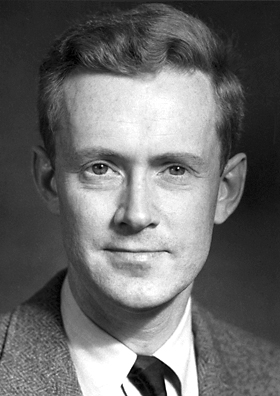
\includegraphics[width=.405\linewidth]{Purcell}

	Пёрселл Эдуард Миллс 


  \label{fig:test1}
\end{minipage}%
\hfill
\begin{minipage}{.5\textwidth}
  \centering
  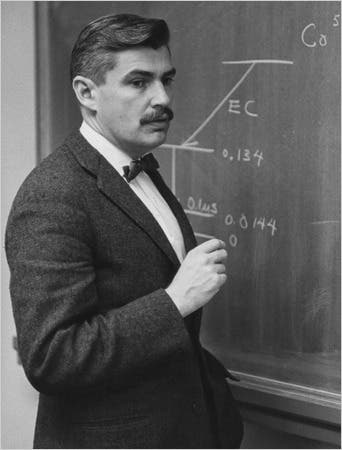
\includegraphics[width=.4377\linewidth]{Pound}

	Паунд Роберт Вивиан
  \label{fig:test2}
\end{minipage}
\end{figure}
\small{
Нобелевские Лауреаты по физике 1952 года <<За развитие новых методов для точных ядерных магнитных измерений и связанные с этим открытия>>, Гарвардский университет.}
\end{frame}

%5	-	Как же её получить?
\begin{frame}
\frametitle{\textcolor{white}{Способ достижения отрицательной температуры}} 
Достижение возможно засчёт передачи энергии системе большей той, которая соотвествует бесконечной температуре. Для большинства систем это невозможно, т.к. их внутренняя энергия также бесконечна.
Однако существуют системы, у которых есть предел внутренней энергии при бесконечной температуры. 
$\lim\limits_{T\to \infty} U(T) = A, A \in \mathbb{R}$
\newline
\newline
Тогда мы можем получить для таких систем состояния с отрицательной температурой.

\end{frame}


%6	-	ограниченность энергии, выстраивание спинов по полю и против
\begin{frame}
\frametitle{\textcolor{white}{Проецирование числовой оси на круг}} 
Станет понятней, если спроецировать числовую ось на круг.

\begin{flushright}
\begin{minipage}{.65\textwidth}
  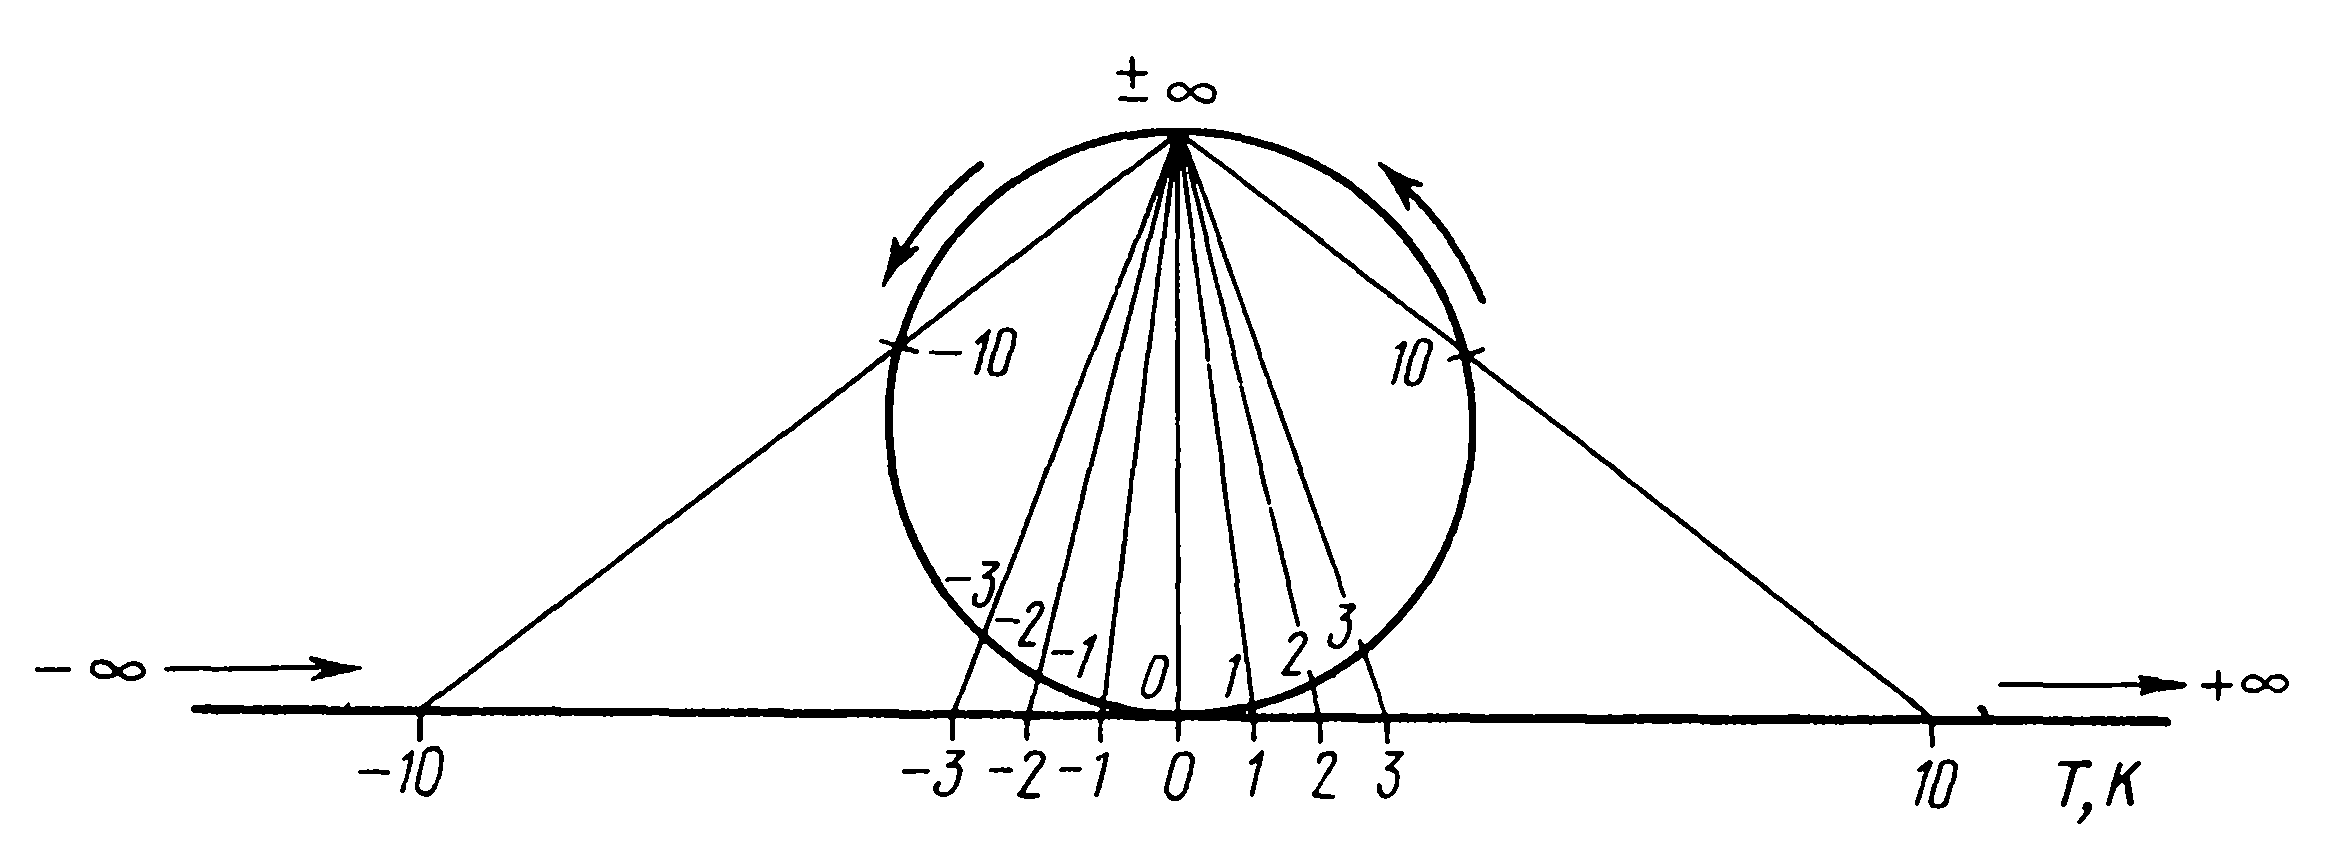
\includegraphics[scale=0.2]{circle}
\end{minipage}

\end{flushright}
Из рисунка видно, что точки $\pm \infty $ совпадают. Если пройти от 0 против часовой стрелки, то мы и получим всю числовую ось. То есть отрицательные температуры находятся <<выше бесконечной температуры>>, а <<не ниже>>, т.е. она горячее, чем при положительных. Более удобная шкала для отрицательных температур будет выглядеть следующим образом: $T^{\ast} = -\frac{1}{T}$
\end{frame}


%7	-	достижимость отрицательной температуры на практике
\begin{frame}
\frametitle{\textcolor{white}{Достижимость отрицательной температуры на практике}} 
%Это то, что я должен буду рассказывать на впв
%Система элементарных магнитов во внешнем магнитном поле. При низкой температуре молекулярные магниты устанавливаются в положение с наименьшой энергией. При сообщении энергии уже не все магниты выстроены по направлению поля, при увеличении температуры распределение становится все более беспорядочным, при $T = + \infty$ частицы распределены по всем энергетическим уровням. Если еще сообщить энергию, то все магниты выстроятся против магнитного поля, что соответвствует отрицательной температуре. 

\begin{figure}
\centering
\begin{minipage}{.5\textwidth}
  \centering
  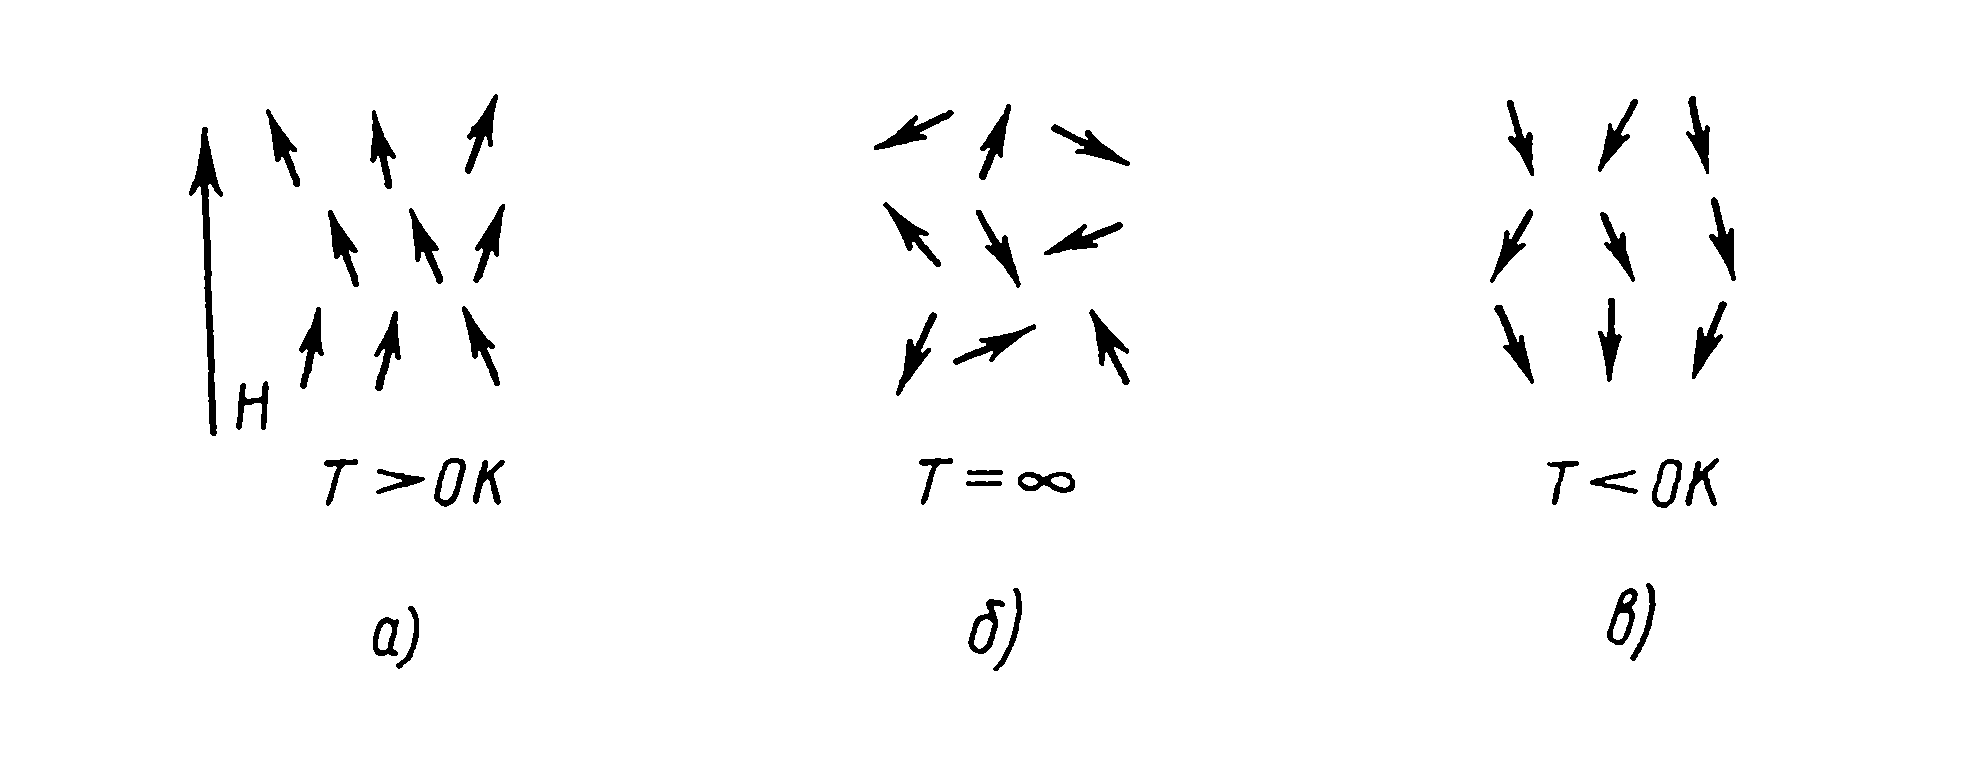
\includegraphics[width=.805\linewidth]{magnete}

	\small{\textit{Система элементарных магнитов во внешнем магнитном поле}}
  \label{fig:test1}
\end{minipage}%
\begin{minipage}{.5\textwidth}
  \centering
  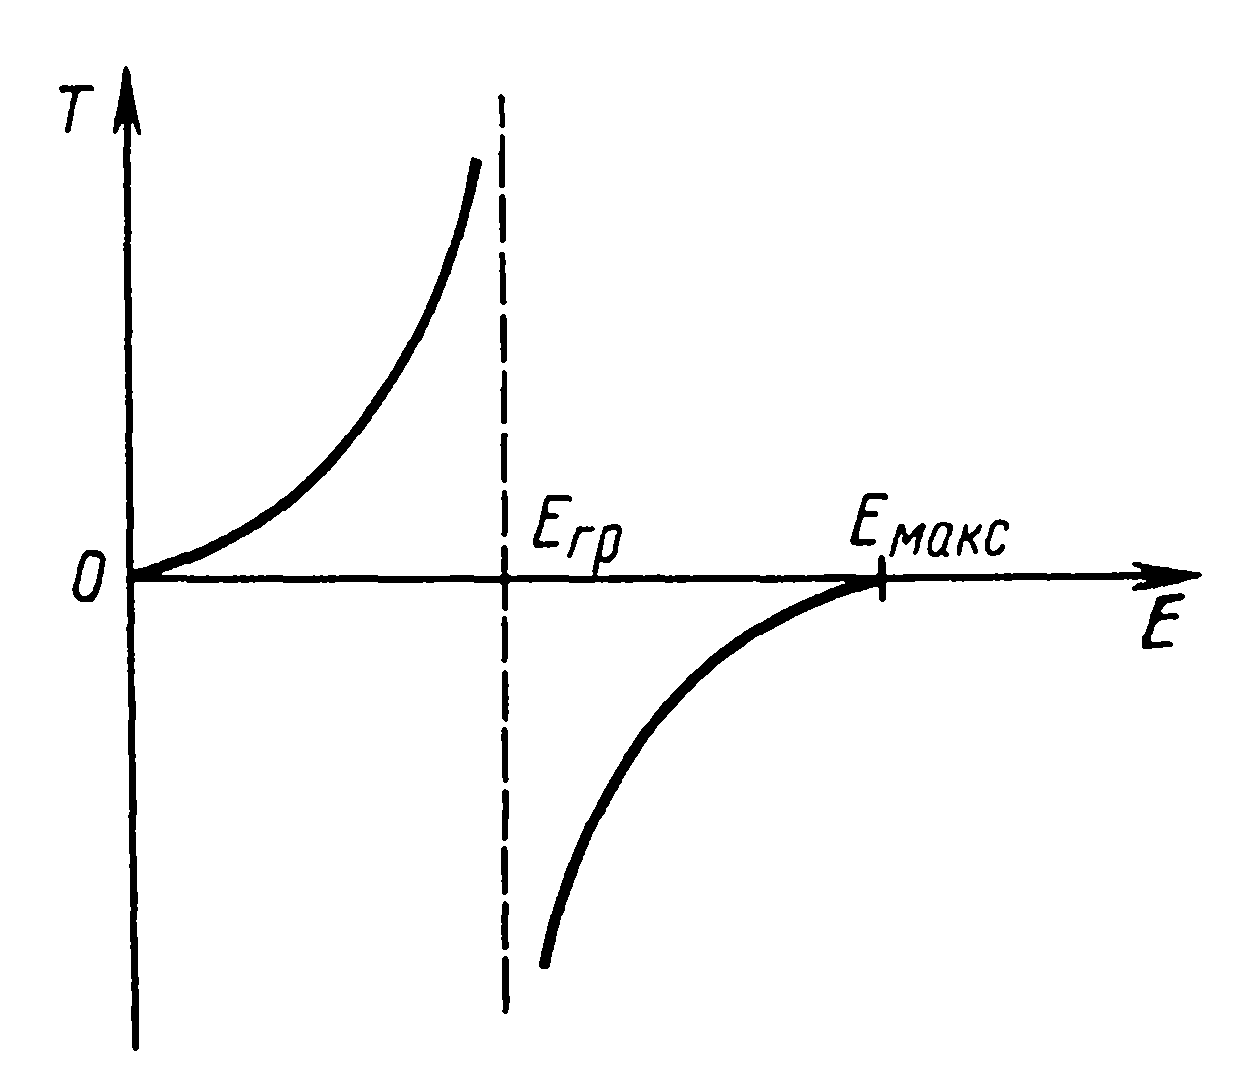
\includegraphics[width=.72\linewidth]{graph}

	\small{\textit{Зависимость внутренней энергии системы от температуры}}
  \label{fig:test2}
\end{minipage}
\end{figure}

Условие, которому соотвествует подобная система:
Энергия термодинамической системы должна иметь конечный предел на бесконечности, а также конечное число энергетических уровней. Система должна быть изолирована от систем, не удовлетворяющих этому условию. 
\end{frame}


\begin{frame}
\frametitle{\textcolor{white}{Начала термодинамики}} 

Второе начало термодинамики в формулировке Каратеодори сохраняется:
Вблизи каждого состояния любой термически однородной системы существуют такие состояния, которые недостижимы из него адиабатным путём. 
То есть существует энтопия как функция её состояния 
\begin{equation}
dS = \frac{\delta Q}{T}
\end{equation}


\vspace{0.16cm}
Второе начало термодинамики для необычных систем при отрицательных температурах:
Невозможен вечный двигатель второго рода, причём это утверждение допускает обращение.
Т.е. в замкнутом круговом процессе при отрицательных температурах ни теплоту нельзя превратить в работу без компенсации (первый элемент), ни работу в теплоту (второй элемент)


\end{frame}

\begin{frame}
\frametitle{\textcolor{white}{Начала термодинамики}} 

Формулировка для любых систем:
Невозможен вечный двигатель второго рода, причём это утверждение не допускает обращения в случае обычных систем и допускает обращение при отрицательных температурах в случае необычных систем.

Основные уравнения и неравенство термодинамики для систем при (T < 0 К) имеют вид:

\begin{equation}
TdS \leqslant dU + \delta A
\end{equation}

\vspace{0.2cm}

Принцип недостижимости абсолютного нуля (если под абсолютным нулём понимать как +0 К, так и -0 К): 
Невозможно с помощью любой, как угодно идеализированной процедуры за конечное число операций охладить любую систему до +0 К или нагреть любую систему до -0 К.
\end{frame}

\begin{frame}
\frametitle{\textcolor{white}{Свойства систем с отрицательными температурами}}
\vspace{0.05cm}
\begin{enumerate}
\item Из (1) следует, что при сообщении теплоты ($\delta Q > 0$), её энтропия уменьшается, система переходит в более упорядоченное состояние.

\item Из (2) можно установить направление перехода тепла при тепловом контакте двух тел с разной температурой. Есть два тела с отрицательным температурами $T_1$ и $T_2$. Пусть от первого тела ко второму перейдёт количество теплоты $\delta Q$ при их контакте. Тогда процесс передачи необратим, получаем: $-\frac{\delta Q}{T_1} + \frac{\delta Q}{T_2} > 0$.
Откуда $T_1 > T_2$, следовательно согласно температурной шкале, тепло переходит от горячего тела к холодному.

\item При отрицательной температуре могут быть проведены различные круговые процессы подобные циклу Карно. Пусть $T_1$ - температура теплоотдатчика, $T_2$ - температура теплоприёмника. Тогда КПД цикла Карно: $\eta = 1 - \frac{T_2}{T_1}$. Температура теплоотдатчика больше, чем теплоприймника, то $T_1 > T_2$, $|T_2| > |T_1|$, $\frac{T_2}{T_1} > 1$ $\rightarrow$ $\eta < 0$.
\item КПД цикла Карно в области отрицательных температур, также меньше 1, то есть этот цикл, как и при положительных температурах поглащает теплоту больше, чем совершает работу.
\end{enumerate}
\end{frame}

\begin{frame}
\frametitle{\textcolor{white}{Устойчивость систем с отрицательными температурами}}
Для нестатических процессов из неравенства (2) получаем:
\begin{equation}
TdS < dU + \delta A
\end{equation}
Откуда следует, что в изолированных системах (U = const, V = const) с T < 0 К равновесие наступает при максимальной энтропии.
Общее условие равновесия при отрицательных температурах: $\Delta S > 0$ или $dS > 0, d^2S > 0$.

Перейдём к независимым переменным:
\begin{equation}
dF > -SdT - pdV
\end{equation}
\begin{equation}
dG > -SdT + Vdp
\end{equation}

\end{frame}

\begin{frame}
\frametitle{\textcolor{white}{Условия устойчивости систем}}
\vspace{0.14cm}
Тогда при термоизохорных процессах получаем:  $\Delta F > 0, \quad dF > 0, \quad d^2F > 0$


А при термоизобарных процессах:  $\Delta G > 0, \quad dG > 0, \quad d^2G > 0 $


Откуда $$\left(\frac{\partial T}{\partial S}\right)_V = \frac{T}{C_V} < 0 , \quad \left(\frac{\partial p}{\partial V}\right)_T  > 0 $$ или 
\begin{equation}
C_V > 0 ,\quad \left(\frac{\partial p}{\partial V}\right)_T  > 0 .
\end{equation}
А также $$\left(\frac{\partial T}{\partial S}\right)_p = \frac{T}{C_p} < 0 ,\quad \left(\frac{\partial p}{\partial V}\right)_S > 0 $$ или 
\begin{equation}
C_p > 0 ,\quad \left(\frac{\partial p}{\partial V}\right)_S > 0 .
\end{equation}
Таким образом, условия устойчивочти равновесных состояний системы с отрицательной температурой выражается неравенствами (6) и (7).
\end{frame}
%8	-	термодинамика систе



\end{document}